%------------------------------
%Setup

\documentclass{beamer}

\makeatletter
\def\beamer@calltheme#1#2#3{%
	\def\beamer@themelist{#2}
	\@for\beamer@themename:=\beamer@themelist\do
	{\usepackage[{#1}]{\beamer@themelocation/#3\beamer@themename}}}

\def\usefolder#1{
	\def\beamer@themelocation{#1}
}
\def\beamer@themelocation{}


\usefolder{Theme}
\usetheme[progressbar=frametitle]{metropolis}
\usepackage{fontspec}      

%------------------------------


%------------------------------
%Cover

\title{Ανάπτυξη εργαλείου για την σχεδίαση παιχνιδιών με την βοήθεια υπολογιστή}
\subtitle{Παρουσίαση πτυχιακής εργασίας}
\date{Μάιος, 2016}
\author[Your Name]{Γιώργος Μιχαηλίδης (3122)
	\\{\small Επιβλέπων: Δρ. Νικόλαος Πεταλίδης}}
\institute{ΤΕΧΝΟΛΟΓΙΚΟ ΕΚΠΑΙΔΕΥΤΙΚΟ ΙΔΡΥΜΑ ΚΕΝΤΡΙΚΗΣ ΜΑΚΕΔΟΝΙΑΣ\\
	ΣΧΟΛΗ ΤΕΧΝΟΛΟΓΙΚΩΝ ΕΦΑΡΜΟΓΩΝ\\
	ΤΜΗΜΑ ΜΗΧΑΝΙΚΩΝ ΠΛΗΡΟΦΟΡΙΚΗΣ ΤΕ}
\titlegraphic{\hfill
\includegraphics[height=1.5cm]{Images/logo_teiser}}

%------------------------------


%------------------------------
%Slides

\begin{document}
	\maketitle
	\begin{frame}{Περιεχόμενα}
		\setbeamertemplate{section in toc}[sections numbered]
		\tableofcontents%[hideallsubsections]
	\end{frame}
	
	\section{Εισαγωγή}
		\begin{frame}{Η ανάγκη δημιουργίας ενός εργαλείου για ανάπτυξη λογισμικού}
			Η διαδικασία ανάπτυξης λογισμικού είναι ακριβή και ο σχεδιασμός γίνεται όλο και πιο σύνθετος και περίπλοκος. Τα έργα γίνονται όλο και πιο απαιτητικά και δαπανηρά. Δημιουργήθηκε η ανάγκη για ένα εργαλείο το οποίο να παρέχει ένα ομοιογενές περιβάλλον για την ανάπτυξη σύνθετων έργων. 
			Ένα \alert{CASE (Computer Aided Software Engineering) tool} είναι ένα λογισμικό-εργαλείο το οποίο απλοποιεί τον κύκλο ανάπτυξης ενός λογισμικού. 		
		\end{frame}		
		\begin{frame}{Κοινές λειτουργίες των Case tools}
			\begin{itemize}
				\item Δημιουργία ροής δεδομένων και μοντέλων οντοτήτων.
				\item Καθιέρωση της σχέσης μεταξύ απαιτήσεων και προτύπων.
				\item Ανάπτυξη του σχεδιασμού σε υψηλό επίπεδο.
				\item Ανάπτυξη λειτουργικών και διαδικαστικών περιγραφών
				\item Ανάπτυξη περιπτώσεων δοκιμών (test cases).	
			\end{itemize}		
		\end{frame}	
		\begin{frame}{Σκοπός της πτυχιακής}
			Σκοπός της πτυχιακής είναι να εξηγήσει σε υψηλό επίπεδο τη σύνδεση και αλληλεπίδραση βασικών υποσυστημάτων τα οποία απαρτίζουν μια
			τυπική μηχανή γραφικών, μαζί με διαγράμματα και παραδείγματα χρήσης του API.
		\end{frame}	
		\begin{frame}{Υλοποίηση}
		Η υλοποίηση χωρίζεται σε δύο μεγάλα μέρη.	
		\begin{itemize}
			\item Τη βιβλιοθήκη \alert{Gem Engine} η οποία περιέχει τις κύριες λειτουργίες και τα υποσυστήματα τα οποία απαρτίζουν τη μηχανή γραφικών όπως είναι, το σύστημα εισόδων και η διαχείριση οθονών.
			\item Tο γραφικό περιβάλλον της μηχανής \alert{Gem IDE} το οποίο προσφέρει οπτική αναπαράσταση των λειτουργιών του \alert{Gem Engine}. Μέσω του \alert{Gem IDE} o χρήστης μπορεί να αποσφαλματώσει το παιχνίδι και να προσθέσει λειτουργίες μέσω γραφικού περιβάλλοντος.
		\end{itemize}
		\end{frame}			
		
	\section{Mηχανές Γραφικών}	
	\begin{frame}{Τι είναι μια μηχανή γραφικών}		
		Στο τομέα του σχεδιασμού παιχνιδιών το πιο διαδεδομένο CASE tool είναι η \alert{μηχανή γραφικών}. Μια μηχανή γραφικών είναι μια σουίτα από επαναχρησιμοποιήσιμα οπτικά εργαλεία, τα οποία βρίσκονται σε ένα ενιαίο περιβάλλον. \cite{gregory2009game}
	\end{frame}
	
	\begin{frame}{Τι παρέχει μια μηχανή γραφικών}		
	\begin{enumerate}
		\item Φωτοαπόδοση σε πραγματκό χρόνο (real time rendering)
		\item Mηχανή φυσικής και εντοπισμς συγκρούσεων (physics and collision detection)
		\item Scripting
		\item Animation
		\item Τεχνητή νοημοσύνη (artificial intelligence)
		\item Δικτύωση (networking)
		\item Παραλληλισμό ενεργειών (multitasking)
		\item Διαχείριση μνήμης
		\item Γράφο σκηνής (scene graph)
	\end{enumerate}
	\end{frame}
		
	\begin{frame}{Ανάπτυξη ηλεκτρονικών παιχνιδιών}
		Ανάπτυξη ηλεκτρονικών παιχνιδιών (game development) ονομάζουμε τη διαδικασία της δημιουργίας ενός παιχνιδιού. Η ομάδα ανάπτυξης μπορεί να κυμαίνεται από ένα άτομο μέχρι μια μεγάλη επιχείρηση.	
	\end{frame}
	
	\begin{frame}{Σχεδιασμός παιχνιδιών}
		Σχεδιασμό παιχνιδιών (game design) ονομάζουμε τον σχεδιασμό και την εφαρμογή τεχνικών αισθητικής στη δημιουργία ενός παιχνιδιού με σκοπό τη διευκόλυνση της αλληλεπίδρασης μεταξύ των παικτών. Οι μηχανές γραφικών χρησιμοποιούνται για σκοπούς δημιουργίας παιχνιδιών.
	\end{frame}
	
	\section{Bιβλιοθήκη}
		
	\begin{frame}{Κύκλος ζωής του πυρήνα}
		\begin{figure}
			\centering
			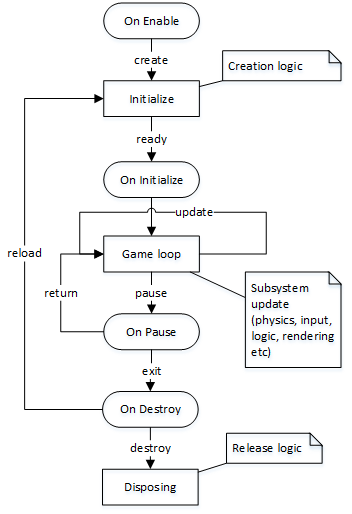
\includegraphics[width=53mm]{Images/core_lifecycle}
		\end{figure}	
	\end{frame}

	\begin{frame}{Φυσική και εντοπισμός συγκρούσεων}
		\begin{figure}			
			\centering
			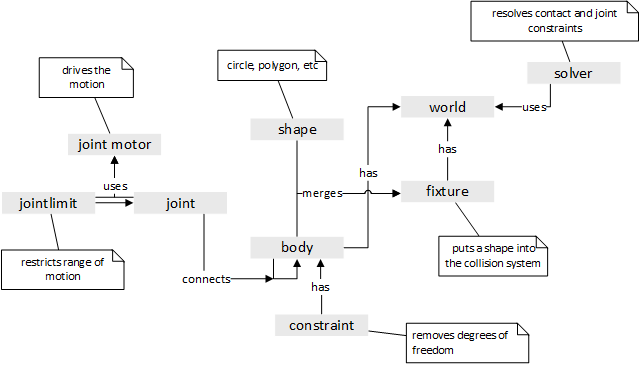
\includegraphics[width=110mm]{Images/physics_engine}
		\end{figure}	
	\end{frame}
			
	\section{Συμπεράσματα}
	\begin{frame}{Επέκταση}
		Ανασκόπηση
	\end{frame}
	
	\plain{Ερωτήσεις;}
		
	\begin{frame}[allowframebreaks]{Βιβλιογραφία}
		
		\bibliography{../Content/bibliography} 
		\bibliographystyle{abbrv}
		
	\end{frame}
	
\end{document}

